\chapter{Adversarial Attack Methodology and Robustness Certification}

\section{Introduction to Adversarial Attacks}

Adversarial attacks are deliberately constructed perturbations to input data that cause an ML model to make incorrect predictions with high confidence. These perturbations are often imperceptible or bounded in norm, but can expose vulnerabilities in the model's internal representations and loss surface geometry.

For sequential models such as the LNN, TCN, and LSTM, adversarial robustness is important, especially in safety-critical applications involving temporal dynamics. Several attacks are implemented in this project, targeting both gradient-accessible and gradient-free contexts, and include both white-box and black-box variants.

Each attack was evaluated under the same conditions, using:
\begin{itemize}
    \item A fixed perturbation budget $\epsilon$.
    \item Normalised data inputs, with identical initial conditions across models.
    \item Denormalised outputs for interpretability and comparison.
\end{itemize}

The metrics used for evaluating adversarial degradation included \textbf{Degradation Ratio}, \textbf{Deviation}, anf \textbf{Local Sensitivity} (Lipschitz constant). For all models/attacks, further explanation of these metrics, numerical results, and qualitative analysis can be found in the evaluation section \ref{chap:evaluation}.

\section{Fast Gradient Sign Method (FGSM)}

The Fast Gradient Sign Method (FGSM) is a single-step adversarial attack first introduced by Goodfellow et al.\cite{goodfellow2015explaining} in 2014. It exploits the local linearity of neural networks by using the gradient of the loss function with respect to the input to perturb the input data in the direction that maximally increases loss.

\subsection*{Mathematical Representation}
Given a model $f_\theta$, a loss function $\mathcal{L}(f_\theta(x), y)$, and a clean input-target pair $(x, y)$, the FGSM adversarial input is constructed as:
\[
x^{\text{adv}} = x + \epsilon \cdot \text{sign} \left( \nabla_x \mathcal{L}(f_\theta(x), y) \right)
\]
where $\epsilon$ controls the perturbation magnitude and $\text{sign}(\cdot)$ is applied elementwise. The method requires only a single forward and backward pass.

This adversarial input is then passed to the model, which produces an adversarial output that is examined.

\subsection*{Implementation Details}
FGSM is implemented in this project using PyTorch's autograd engine. The input tensor is marked with \texttt{requires\_grad=True} and gradients are computed by backpropagating through the MSE loss between model output and the clean target sequence. The sign of the gradient is scaled by $\epsilon$ and added to the input.

\begin{lstlisting}[language=Python, caption={FGSM adversarial attack implementation}]
loss = F.mse_loss(model(x), y)
loss.backward()
perturbation = epsilon * x.grad.sign()
x_adv = x + perturbation
\end{lstlisting}

\subsection*{Attack Design Reflection:}  
FGSM is efficient but limited, as it assumes linearity and is easy to defend against with basic regularisation, so was used as a baseline attack method.

\section{Projected Gradient Descent (PGD)}

The PGD attack is an iterative extension of FGSM and is regarded as one of the stronger first-order adversaries in adversarial machine learning. Proposed by Madry et al. \cite{madry2018towards}, PGD performs multiple small steps of perturbation in the direction of the loss gradient, updating the input to increase model error. After each step, the perturbed input is projected back onto an $\ell_p$ ball of fixed radius $\varepsilon$ centered around the original input. The $\ell_p$ ball defines the set of allowable perturbations under a given norm constraint. For instance, the $\ell_\infty$ ball constrains each individual input dimension to change by no more than $\varepsilon$, and the $\ell_2$ ball bounds the overall Euclidean distance of the perturbation. This constraint ensures that the adversarial input remains imperceptibly close to the original, preserving its semantics and attempting to fool the model.

\subsection*{Mathematical Representation}
Given an input $x$ and perturbation budget $\epsilon$, PGD initializes the adversarial input as $x_0^{\text{adv}} = x + \delta$ (with $\delta$ small or random), and iteratively updates it as follows:
\[
x_{t+1}^{\text{adv}} = \Pi_{B_\epsilon(x)} \left( x_t^{\text{adv}} + \alpha \cdot \text{sign}\left( \nabla_x \mathcal{L}(f_\theta(x_t^{\text{adv}}), y) \right) \right)
\]
Here, $\Pi_{B_\epsilon(x)}$ denotes the projection onto the $\ell_\infty$ ball centered at $x$ with radius $\epsilon$, and $\alpha$ is the step size.

\subsection*{Implementation Details}
The attack was implemented using a fixed number of iterations (10). In each step, the model first performed a forward pass on the current adversarial input. Then, 
the loss was computed and backpropagated to obtain input gradients. Finally the adversarial input was updated using the signed gradient and clipped back to the $\epsilon$-bounded domain. This process is then repeated, using the new adversarial input as the starting point.

\begin{lstlisting}[language=Python, caption={PGD Attack Loop (Simplified)}]
for _ in range(num_iter):
    output = model(x_adv)
    loss = F.mse_loss(output, target)
    loss.backward()
    with torch.no_grad():
        x_adv += alpha * x_adv.grad.sign()
        perturbation = torch.clamp(x_adv - x_orig, min=-epsilon, max=epsilon)
        x_adv = torch.clamp(x_orig + perturbation, min, max).detach().requires_grad_()
\end{lstlisting}

\subsection*{Design Choices}
\begin{itemize}
    \item \textbf{Step size $\alpha$:} Set as $0.01$ after empirical tuning to balance convergence and perturbation spread.
    \item \textbf{Projection radius $\epsilon$:} Fixed at $0.05$ to match FGSM budget for fair comparison.
    \item \textbf{Clipping bounds:} Enforced to retain normalised input range and ensure comparability with clean evaluations.
\end{itemize}

Unlike FGSM, PGD exposes high-curvature regions of the loss surface. The extent to which a model resists PGD steps provided insight into the local geometry of its input-output mapping.

\section{DeepFool-Inspired Directional Attack}

FGSM and PGD rely on sign-based or norm-bounded perturbations and, whilst effective, can be inefficient in identifying the minimal perturbation required for misprediction. DeepFool, introduced by Moosavi-Dezfooli et al. \cite{moosavi2016deepfools}, aims to iteratively approximate the closest decision boundary in input space. Since it was originally designed for classification, a novel modified version was implemented here to exploit the gradient direction of loss for regression.

\subsection*{Mathematical Representation}
In its original form, DeepFool linearises the classifier around the current point and computes the minimal step in the direction of the gradient that crosses the decision boundary. In the adaptation for regression, the perturbation is applied directly in the normalised direction of the loss gradient, without projection.

The update rule is given by:
\[
x^{\text{adv}} = x + \eta \cdot \frac{\nabla_x \mathcal{L}(f(x), y)}{ \| \nabla_x \mathcal{L}(f(x), y) \|_2 + \delta }
\]
where $\eta$ is a scalar perturbation magnitude and $\delta$ is a small stabilisation term to prevent division by zero.

\subsection*{Implementation Summary}
The attack was implemented using a single or few iterations, computing the raw gradient of the loss with respect to the input and stepping along the normalised direction. Unlike PGD, no projection or clipping was applied. This was chosen to explore worst-case directional drift.

\begin{lstlisting}[language=Python, caption={Directional (DeepFool-like) Gradient Attack}]
loss = F.mse_loss(model(x), y)
loss.backward()
gradient = x.grad.data
perturbation = eta * gradient / (torch.norm(gradient) + epsilon)
x_adv = x + perturbation
\end{lstlisting}

\subsection*{Design Considerations}
\begin{itemize}
    \item \textbf{Normalisation:} The gradient was normalised using $\ell_2$ norm rather than using the sign, to emulate the boundary-seeking nature of DeepFool.
    \item \textbf{No projection:} This allowed the perturbation to fully reflect the underlying geometry of the loss surface, rather than artificially constraining it.
    \item \textbf{Step size tuning:} $\eta$ was selected via a sweep, typically in the range $[0.01, 0.05]$.
\end{itemize}

This attack highlights structural vulnerability that simpler norm-bounded methods could have missed. For continuous dynamics models like the LNN, sensitivity to gradient direction (rather than just amplitude) was observed.

\section{Simultaneous Perturbation Stochastic Approximation (SPSA)}

The Simultaneous Perturbation Stochastic Approximation (SPSA) attack is a gradient-free adversarial method designed for scenarios where gradient information is inaccessible, unreliable, or expensive to compute. Originally proposed for optimisation in noisy environments, SPSA estimates gradients by evaluating the function along random perturbation directions.

SPSA is therefore a suitable candidate for attacking models with non-differentiable components or highly unstable gradient behaviour. These are conditions often encountered in ODE-based or discretised models like the LNN.

\subsection*{Mathematical Representation}
Let $x \in \mathbb{R}^d$ be the input and $\mathcal{L}$ the loss function. At each iteration, SPSA perturbs $x$ in a randomly sampled direction $\Delta \sim \{\pm 1\}^d$, and estimates the gradient as:
\[
\hat{g}_i = \frac{\mathcal{L}(x + \sigma \Delta) - \mathcal{L}(x - \sigma \Delta)}{2 \sigma} \cdot \Delta_i
\]
The input is then updated via:
\[
x^{\text{adv}}_{t+1} = x^{\text{adv}}_t + \alpha \cdot \text{sign}(\hat{g})
\]
Here, $\sigma$ controls the scale of the finite difference, and $\alpha$ is the step size. The sign function ensures robustness against outliers in the gradient estimate.

\subsection*{Design Choices}
In this project, the SPSA attack is implemented using binary random perturbation vectors $\Delta$, that are sampled independently at each iteration. Forward passes are executed twice per iteration to estimate the directional gradient. Once calculated, updates are projected back to an $\ell_\infty$ ball of radius $\epsilon$ around the original input.

\begin{lstlisting}[language=Python, caption={Simplified SPSA implementation}]
for _ in range(num_iter):
    delta = torch.randint_like(x, low=0, high=2) * 2 - 1  # + or - 1 vector
    loss_plus = loss_fn(model(x + sigma * delta), y)
    loss_minus = loss_fn(model(x - sigma * delta), y)
    grad_estimate = (loss_plus - loss_minus) / (2 * sigma) * delta
    x = x + alpha * grad_estimate.sign()
\end{lstlisting}

\subsection*{Reflections on Robustness}
\begin{itemize}
    \item \textbf{Gradient-free limitation:} SPSA is powerful when gradients are inaccessible, but its convergence is sensitive to $\sigma$ and batch size.
    \item \textbf{Hyperparameter sensitivity:} Choosing appropriate $\alpha$ and $\sigma$ values is important. Small values cause the gradient estimate to vanish and large values cause the model to overshoot the adversarial direction.
    \item \textbf{Noise tolerance:} The LNN's time-averaged dynamics and implicit smoothness provided resilience against the perturbations introduced by SPSA.
\end{itemize}

The stochastic nature of this attack mirrors real-world adversarial conditions, where inputs may be corrupted by structured or unstructured noise.

\section{Time-Warping Attack}

Unlike traditional adversarial attacks that modify the magnitude of input features, the time-warping attack alters the temporal structure of the input sequence. This approach is motivated by the fact that many sequence models implicitly assume uniform temporal spacing, and small distortions in timing can have disproportionately large effects on prediction accuracy.

\subsection*{Conceptual Basis}
For trajectory prediction, a time-warping attack perturbs the relative spacing between consecutive time steps, modifying the speed (sampling rate) of the underlying system without changing the actual trajectory points themselves. This is effective on models with strong temporal priors, such as recurrent or ODE-based networks.

\subsection*{Mathematical Representation}
Let $x = [x_0, x_1, \dots, x_{T-1}]$ be a sequence of length $T$. A warping function $w: \{0, 1, \dots, T-1\} \to \mathbb{R}$ maps each time index to a new location. After applying interpolation to enforce fixed-length output, the warped sequence becomes:
\[
x^{\text{warp}}_t = x(w(t)), \quad \text{where } w(t) = t + \epsilon \cdot \sin\left( \frac{2\pi t}{T} \right)
\]
Here, $\epsilon$ determines the amplitude of the distortion. Interpolation (e.g. linear or cubic) is used to ensure that the resulting sequence remains aligned with the original frame size.

\subsection*{Implementation Strategy}
The attack is implemented in this project by generating control points across the time domain and applying sinusoidal displacements to simulate acceleration and deceleration patterns. The perturbed sequence is then interpolated back to the original length.

\begin{lstlisting}[language=Python, caption={Example Time-Warping Attack Function}]
def warp_sequence(x, epsilon, num_control_points):
    time = np.linspace(0, 1, len(x))
    warp = time + epsilon * np.sin(2 * np.pi * time)
    return interpolate_sequence(x, warp)
\end{lstlisting}

\subsection*{Design Choices}
The perturbation amplitude ()$\epsilon$) is bounded to ensure the warped sequence remained physically plausible and temporally ordered. Linear interpolation is used for stability, since higher-order methods introduce numerical artefacts that empirically degrade learning reproducibility. In addition, the attack is architecture-neutral (since it doesn't require gradient access).

The ability of the continuous-time model (LNN) to handle temporal distortions without significant degradation shows a key advantage. LNNs maintain robustness when underlying assumptions about when those features arrive is attacked.

\section{Continuous-Time Perturbation Attack}

The continuous-time perturbation attack is a novel technique designed specifically for models with internal time dynamics, such as the Liquid Neural Network (LNN). Unlike discrete attacks which perturb input values directly, this method injects structured noise into the temporal dynamics governing the state evolution of the system. This is conceptually aligned with adversarial strategies in control theory and differential equation modelling.

\subsection*{Motivation}
In ODE-based models, the output is not solely a function of discrete inputs, but rather of how internal states evolve over time in response to those inputs. Small perturbations to the continuous-time signal (especially during critical integration intervals) can lead to disproportionately large shifts in the terminal state. The attack is designed to evaluate this phenomenon.

\subsection*{Mathematical Representation}
Given an input sequence $x(t)$ sampled at discrete steps, and a model defined by the differential equation:
\[
\frac{dv}{dt} = F(v, x(t))
\]
the adversarial version modifies $x(t)$ into $x^{\text{adv}}(t)$ by injecting structured noise across all integration intervals, effectively perturbing the right-hand side of the ODE during its internal solver steps.

The adversarial input is constructed as:
\[
x^{\text{adv}}(t_i) = x(t_i) + \delta_i, \quad \delta_i \sim \mathcal{U}(-\epsilon, \epsilon)
\]
where perturbations $\delta_i$ are constrained within a norm bound but applied at each ODE unfold step.

\subsection*{Implementation Details}
This attack is implemented by modifying the input sequence across all ODE solver substeps inside the \texttt{forward} method of the LNN. Unlike standard attacks, which treat input as static, this attack dynamically perturbs the input during internal time integration. The same idea was adapted for discrete models (LSTM, TCN) for comparison, by injecting noise at each time step only once.

\begin{lstlisting}[language=Python, caption={Continuous-Time Perturbation Injection}]
for unfold in range(self.ode_unfolds):
    perturbed_input = inputs + torch.empty_like(inputs).uniform_(-epsilon, epsilon)
    # Proceed with dynamics update using perturbed_input
\end{lstlisting}

\subsection*{Design Choices}
This attack is the only one in the study that targets the solver trajectory itself, not just the input points. For comparability between the LNN and non-ODE models, the same noise patterns were applied to LSTM and TCN (but only once per timestep). For the LNN, they were applied across all ODE unfolds.Uniform noise perturbation shape was used instead of Gaussian to allow strict $\ell_\infty$ control.

This attack probes the intrinsic robustness of models whose internal computations are sensitive to continuous dynamics. The results illustrate that while the LNN offers meaningful protection at low perturbation levels, it remains vulnerable to adversarial trajectories that disrupt the time integration process itself.

\section{Summary of Attack Design and Implementation Decisions}

This subsection consolidates the key methodological choices made across the six adversarial attacks implemented in this study.

\subsection*{Attack Categories and Coverage}
\begin{table}[H]
\centering
\begin{tabular}{|l|c|c|c|}
\hline
\textbf{Attack} & \textbf{Gradient Access} & \textbf{Perturbation Type} & \textbf{Temporal Sensitivity} \\
\hline
FGSM & White-box & Value-based (single-step) & Low \\
PGD & White-box & Value-based (multi-step) & Medium \\
DeepFool-inspired & White-box & Directional / Unbounded & Medium \\
SPSA & Black-box & Value-based (stochastic) & Medium \\
Time-Warping & Gradient-free & Time axis distortion & High \\
Continuous-Time Perturbation & White-box & Internal ODE injection & Very High \\
\hline
\end{tabular}
\caption{Overview of attack types and model sensitivities.}
\label{tab:attack_summary}
\end{table}

\subsection*{Implementation Consistency}
All attacks adhere to a common evaluation pipeline.
The same spiral-based input sequence is used across all models and attacks, and inputs are normalised using the same statistics as during training. Model outputs are denormalised before computing performance metrics. The perturbation budgets ($\epsilon$) are also standardised across comparable attacks (typically 0.05).

\subsection*{General Attack Design Considerations}
\begin{itemize}
    \item \textbf{Reproducibility:} Random seeds are fixed for all stochastic attacks (SPSA, time-warping) to ensure consistent comparison.
    \item \textbf{Numerical Stability:} Small constants ($\delta = 10^{-8}$) are added in division and normalisation steps to prevent undefined behaviour.
    \item \textbf{Model Adaptation:} While some attacks are originally developed for classification or discrete tasks, each was carefully adapted to suit regression-based, sequence-oriented prediction.
\end{itemize}

\section{Certified Robustness Analysis of the LNN via Interval Bound Propagation}

One of the core contributions of this work is the application of certified robustness techniques to Liquid Neural Networks (LNNs), a model class whose temporal dynamics pose unique challenges to formal analysis. While LNNs have demonstrated strong empirical performance on continuous time-series tasks, their verification under perturbations remains largely unexplored in the literature. In this section, we investigate the provable robustness of the trained LNN using \texttt{auto\_LiRPA} \cite{autoLiRPA2022}, a state-of-the-art library for neural network bound propagation and formal verification.

\subsection*{Methodology}

To assess the model's stability under input perturbations, we employ \emph{Interval Bound Propagation} (IBP), a forward method which computes tight, conservative bounds on a model's output when subjected to norm-bounded adversarial noise. Specifically, given a test input \( x_0 \), we define an \(\ell_\infty\) perturbation set \( \mathcal{B}_\epsilon(x_0) = \{x : \|x - x_0\|_\infty \leq \epsilon\} \). IBP then propagates the resulting input interval through the model’s layers to produce lower and upper bounds \( [\underline{f}(x), \overline{f}(x)] \) on the output across the entire input region.

This approach is particularly suitable for LNNs due to its architectural agnosticism and compatibility with continuous-time formulations, and represents, to the best of our knowledge, the first application of certified bound analysis to a liquid neural model. The experimental results in this section are derived from a single representative input sequence drawn from the validation set.

\subsection*{Certified Output Bounds}

Figure~\ref{fig:lnn_ibp_bounds} visualises the certified output interval for dimension 0 of the LNN's prediction across the temporal horizon. The solid blue curve represents the original output trajectory of the LNN on the unperturbed input, while the shaded region denotes the certified range of possible outputs under all admissible perturbations with \( \epsilon = 0.1 \). Notably, for the majority of the sequence, the output remains well-contained within the certified bounds, implying that the model's prediction is provably stable to small variations in the input. However, there is a clear increase in bound looseness in the latter part of the trajectory (timestep 400 onwards), indicating a region of greater uncertainty and higher sensitivity.

\begin{figure}[H]
    \centering
    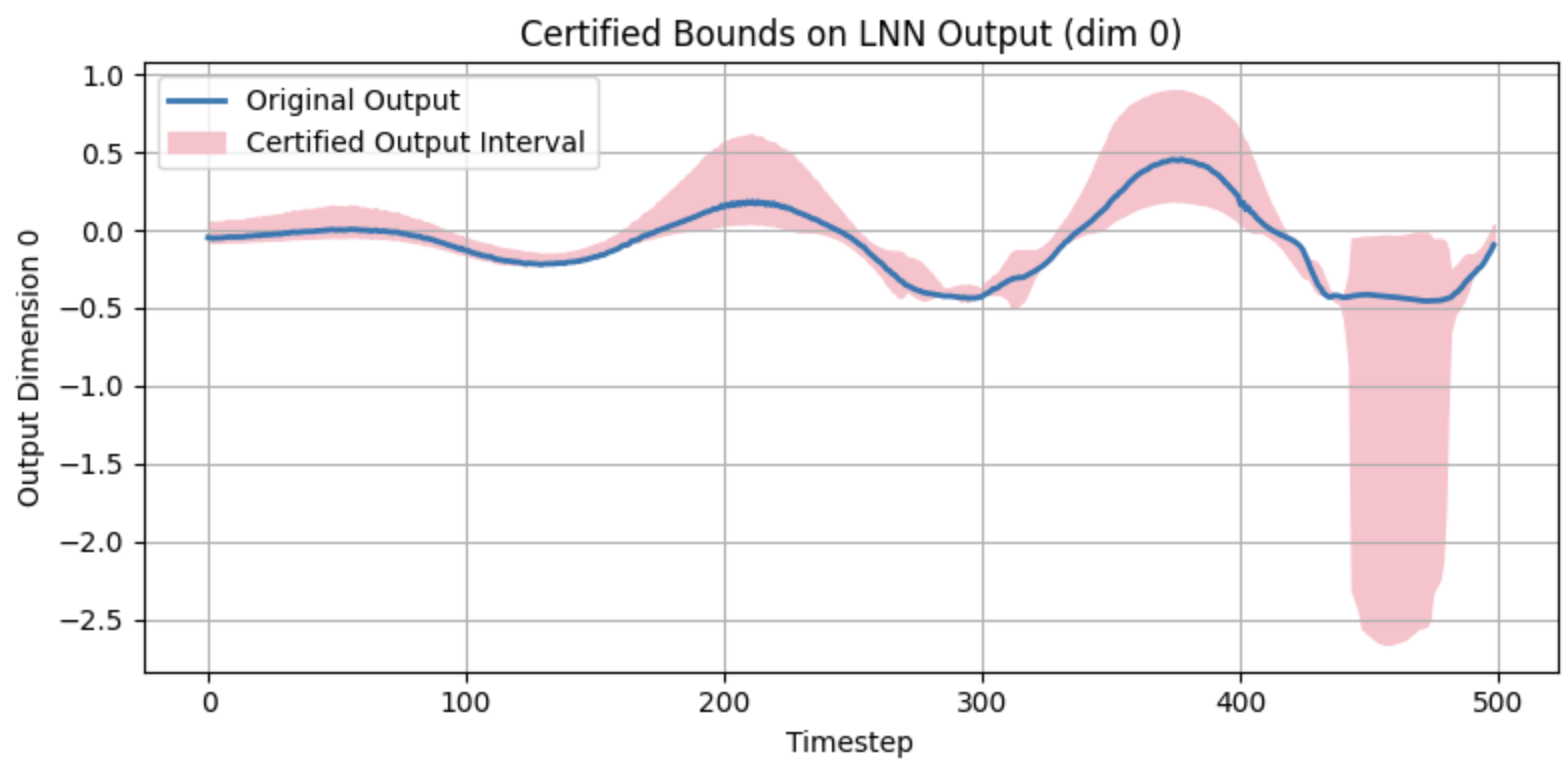
\includegraphics[width=0.9\linewidth]{img/auto_lirpa_lnn_certified_bounds.png}
    \caption{Certified output bounds for LNN prediction on dimension 0, computed using IBP via \texttt{auto\_LiRPA}. The blue line denotes the nominal output; the pink region denotes the certified interval over \( \ell_\infty \)-bounded perturbations.}
    \label{fig:lnn_ibp_bounds}
\end{figure}

\subsection*{Bound Width Dynamics}

To gain insights into where and when the LNN exhibits greater susceptibility to perturbation, we measure the width of the certified bounds over time. Figure~\ref{fig:bound_width_plot} presents the bound width (computed as \( \overline{f}(x) - \underline{f}(x) \)) separately for each output dimension. The certified intervals vary significantly in both magnitude and temporal structure. In particular, dimension 0 shows sharp spikes in bound width near timesteps 300 and 450, reaching values above 20. These spikes align with regions where the underlying dynamics of the LNN are more nonlinear or where hidden states exhibit rapid transitions.

The bound width in dimension 1, while generally smaller in amplitude, remains elevated throughout the sequence, suggesting a persistent direction of vulnerability in the output space. This observation aligns with adversarial attack results, where perturbations were more effective when targeting dimension 1.

\begin{figure}[H]
    \centering
    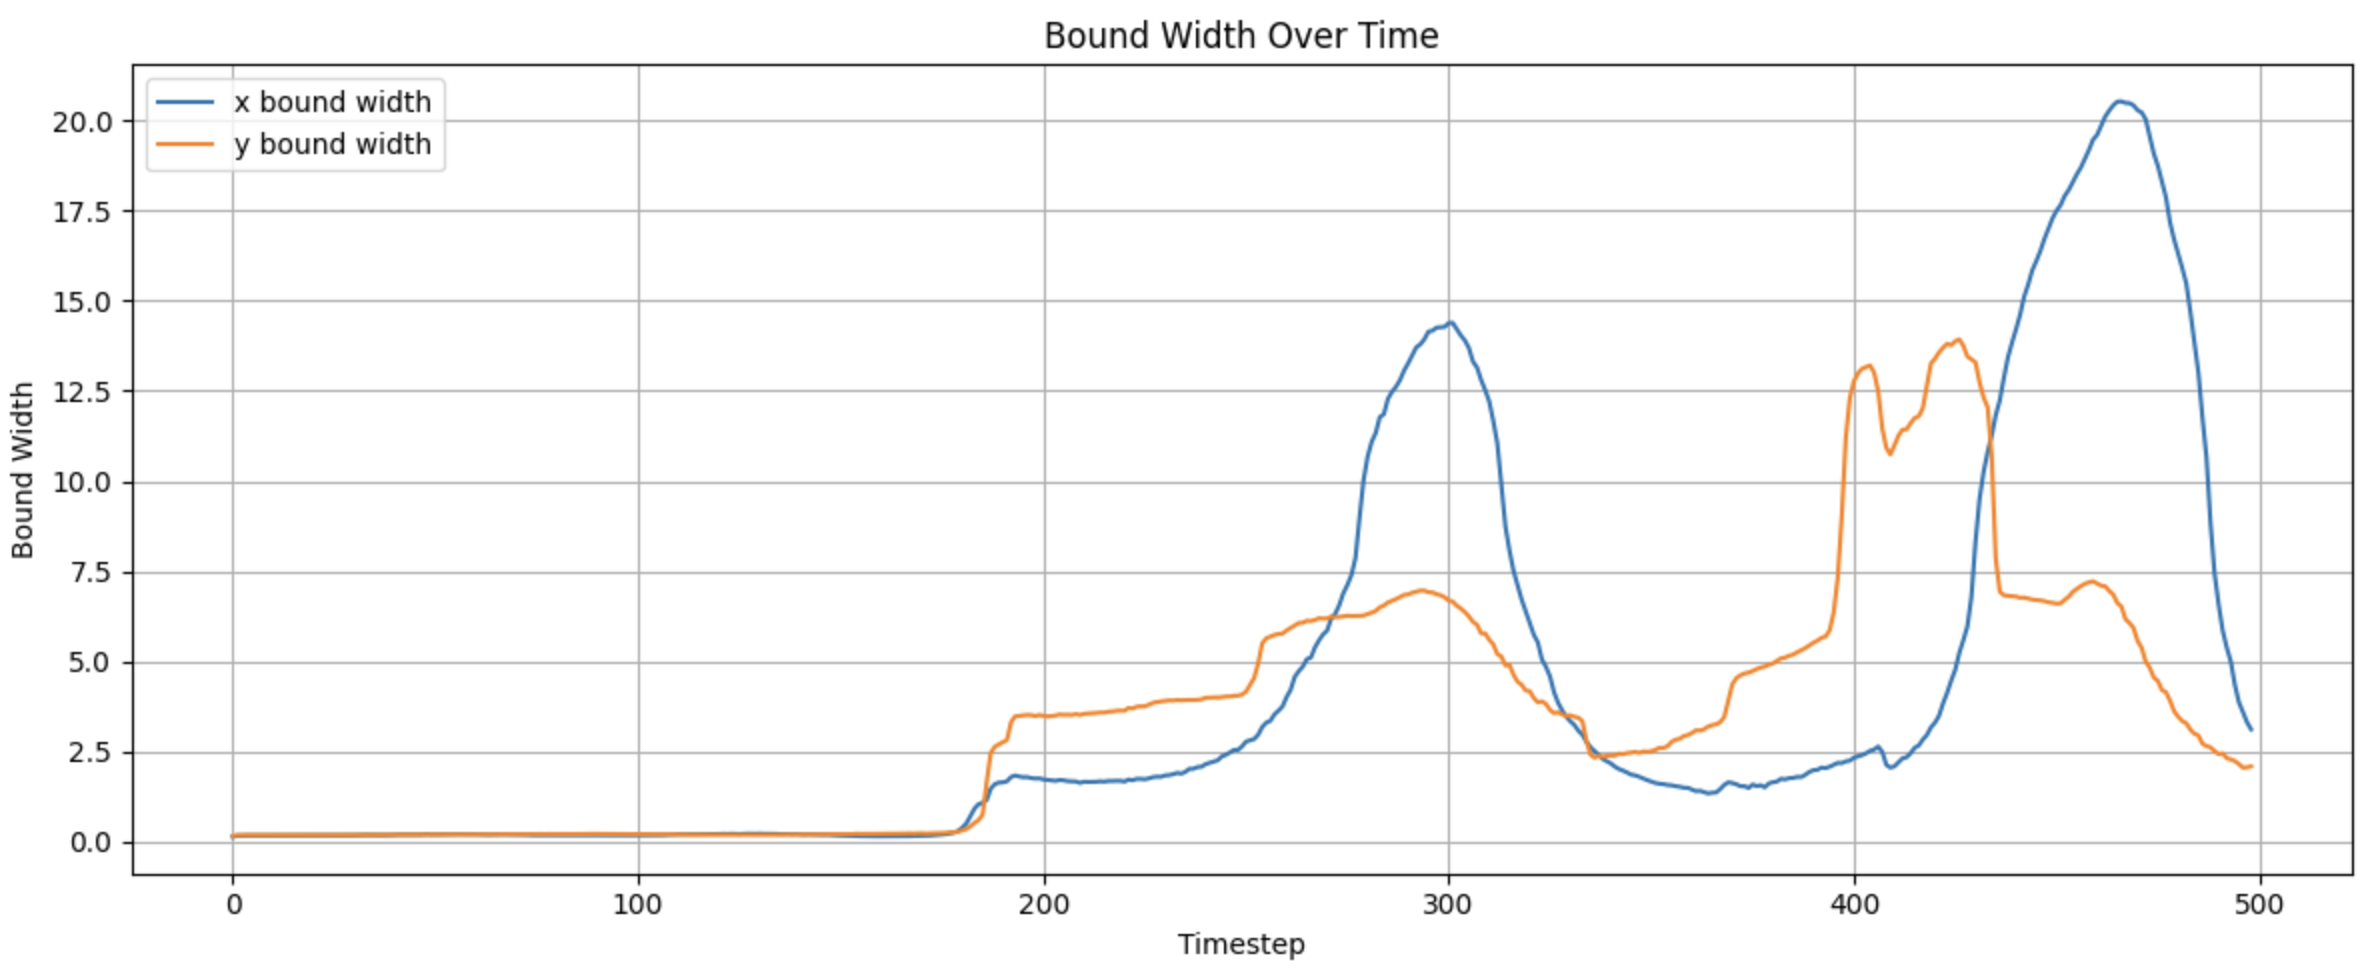
\includegraphics[width=0.9\linewidth]{img/bound_width_over_time.png}
    \caption{Evolution of certified output bound width over time, for both output dimensions of the LNN. Spikes in width correspond to higher uncertainty or sensitivity in the model's output.}
    \label{fig:bound_width_plot}
\end{figure}

\subsection*{Discussion}

These results highlight two key findings. First, the use of IBP enables formal robustness guarantees for LNNs. Second, the certified bounds demonstrate a non-uniform sensitivity profile, with certain regions of the prediction horizon exhibiting high confidence (tight bounds), and others reflecting instability (loose bounds). This fine-grained temporal analysis offers insight into where robustness training or architectural regularisation may be most effective. Future work could extend this framework using tighter bounds (e.g. CROWN-IBP) or adversarial training to actively reduce the width of certified intervals.